\documentclass[12pt,letterpaper]{article}

\usepackage{cvpr}
\usepackage{times}
\usepackage{epsfig}
\usepackage{graphicx}
\usepackage{amsmath}
\usepackage{amssymb}
\usepackage{subfig}
\usepackage{appendix}

% Include other packages here, before hyperref.

% If you comment hyperref and then uncomment it, you should delete
% egpaper.aux before re-running latex.  (Or just hit 'q' on the first latex
% run, let it finish, and you should be clear).
\usepackage[breaklinks=true,bookmarks=false]{hyperref}

\cvprfinalcopy % *** Uncomment this line for the final submission

\def\cvprPaperID{****} % *** Enter the CVPR Paper ID here
\def\httilde{\mbox{\tt\raisebox{-.5ex}{\symbol{126}}}}

% Pages are numbered in submission mode, and unnumbered in camera-ready
%\ifcvprfinal\pagestyle{empty}\fi
\setcounter{page}{1}
\begin{document}

%%%%%%%%% TITLE
\title{Regularized Deep Learning in High Energy Physics}

\author{Josh Gartman\\
Northeastern University\\
Boston, MA\\
{\tt\small gartman.j@husky.neu.edu}
% For a paper whose authors are all at the same institution,
% omit the following lines up until the closing ``}''.
% Additional authors and addresses can be added with ``\and'',
% just like the second author.
% To save space, use either the email address or home page, not both
}

\maketitle
%\thispagestyle{empty}

%%%%%%%%% ABSTRACT
\begin{abstract}
  Recent research has explored the uses of deep learning in high energy physics.  Deep learning methods have shown great promise in particle classification tasks.  Typically for these methods to be successful a large training set is required.  In this work we apply deep learning methods using a regularized neural network and a training set of limited size.  Results of deep and shallow networks trained with high and low level features are compared.
\end{abstract}

%%%%%%%%% BODY TEXT
\section{Introduction}
Recent years have seen a dramatic increase in the popularity of deep neural networks.  These networks have shown improved performance over existing methods in diverse areas such as computer vision, speech recognition, and text analysis.  Multiple hidden layers and non-linear activations allow deep networks the flexibility to model complex functions more efficiently and with better generalization that their shallow counterparts.  The use of shallow neural networks has been common practice in high energy physics since the 1980's.  An important application of these networks is in classifying the subatomic particles produced by collisions at particle accelerators \cite{Abreu:1992jp}.

At particle accelerators like the Large Hadron Collider, located outside Geneva Switzerland, protons are accelerated to nearly the speed of light by powerful magnets and then smashed together with the resulting collisions observed by a series of detectors.  At high enough energies rare and unstable particles can be produced.  The data from these collisions, including the speed and trajectories of the resulting particles, can then be input to machine learning algorithms to classify the particles themselves into categories such as bosons or leptons.  Improved machine learning algorithms would have two important benefits.  Firstly, better classification accuracy can improve the chances of correctly classifying a potentially rare or undiscovered particle.  Secondly, improved algorithms can learn on smaller training sets.  Although training data may be created by computer simulation it can be computationally expensive to produce and unwieldy to use.  Smaller training sets allow for models to be trained more quickly while limiting model size.  The goal of this paper is to apply regularized deep learning to datasets of limited size while maintaining or improving classification accuracy when compared to shallow networks.

A recent example of the use of machine learning in high energy physics is in the search for decays of the Higgs Boson directly into fermions at the LHC.  Evidence consistent with the decay of the Higgs particle into two fermionic tau leptons has been seen in data collected at the LHC but current methods lack the statistical power to cross the standard threshhold for claims of discovery \cite{pmlr-v42-cowa14}.  Observing the $H \rightarrow \tau^+ \tau^-$ decay would provide further verification that the Standard Model of particle physics is an appropriate description of the behavior of sub-atomic particles.

\subsection{Related Work}

Shallow networks have been used for decades in particle classification problems but only recently has the use of deep networks been explored.  Baldi et. al. \cite{Baldi:2014kfa}\cite{Baldi:2014pta} apply deep learning to several high energy physics particle classification tasks.  First in \cite{Baldi:2014kfa}, the authors investigate the performance of deep classifiers in detecting the production of the Higgs boson and separately their performance in classifying the production of super-symmetric charged particles that decay to W bosons.  They observed that deep networks utilizing low level data and high level derived features give improved performance over shallow networks trained with the same features.  In the Higgs production task the classifiers performance was not improved by the inclusion of the high level features indicating that the network was able to learn a representation of these features simply from the low level raw input data.  However, in the super-symmetry task the inclusion of high level features led to improved performance making it difficult to generalize whether deep learning can learn representations of these high level features for all particle physics datasets.  Both datasets were of similar size, containing roughly 10 millions training examples with about 30 features for each example.  

In \cite{Baldi:2014pta} the authors focus on the previously described task of searching for the decay of the Higgs into two tau leptons.  Their data set was very large, consisting of 80 million examples. They compare the performance of deep and shallow networks in detecting the decay using combinations of both high and low level features.  Results indicate that deep networks outperform shallow networks even in the case where the shallow network was trained with the full feature set and the deep network was only given the low level features.

\subsection{Overall Approach}

One of the main difficulties with training neural networks is that they can be prone to overfitting.  To address this $L_2$ regularization and dropout were explored.  In \cite{Baldi:2014pta} the authors observed that regularization methods did not not improve their results, speculating that because of the size of their training set the main challenge their model faced was learning rather than preventing overfitting.  Another challenge of training deep neural networks is optimizing hyper-parameters such as the learning rate, number of hidden layers, and number of units per hidden layer.  Because training a neural network is a very computationally expensive procedure it is beneficial to optimize hyper-parameters as efficiently as possible.  In grid search the network is trained repeatedly with different pre-determined values of the hyper-parameters.  Grid search can be computationally wasteful since it does not focus the search on a space of hyper-parameters likely to give the best results.  A Bayesian hyper-parameter optimization procedure is able to use past evaluations of the model to select hyper-parameters most likely to give the best performance which can save valuable computation time.  Many of the recent successes in deep learning can also be traced back to advances in gradient based optimization methods as well as the activation functions used in the networks hidden layers.

\section{Technical Details of Approach}

The following subsections describe in detail the components of the model. 

\subsection{Hyper-parameter Optimization}
The large computational resources that must be spent to train machine learning models such as neural networks can make hyper-parameter optimization difficult.  The advantage of a Bayesian hyper-parameter optimization approach is that the choice of hyper-parameters to evaluate can be made so as to give the best chance of improving the models performance. A Bayesian optimization begins by defining the function to be optimized as being drawn from a Gaussian process prior and then maintaining a posterior distribution for this function as observations are made. In Snoek et. al. \cite{Snoek:2012:PBO:2999325.2999464} the authors describe the model as follows.  The objective function $f(x)$ is drawn from a GP prior and observations are of the form $\{x_n,y_n\}_{n=1}^N$ where $y_n \sim N(f(x_n), \nu)$ and $\nu$ is the variance of noise in the function observations.  The GP prior and the data observations induce a posterior over function. After $f(x)$ is evaluated for a given set of inputs an acquisition function $a : \chi \rightarrow R^+$ is used to try and find a new setting of parameters most likely to minimize the objective.  Because of the properties of a Gaussian Process the acquisition function that gives the greatest expected improvement has a closed form.  This can be derived as:

$a_{EI}(x:{x_n,y_n}, \theta)= \sigma(x;{x_n,y_n},\theta) (\gamma(x) \Phi(\gamma(x)) + N(\gamma(x)))$


$\gamma(x) = \frac{f(x_{best}) - \mu(x;{x_n,y_n}, \theta)}{\sigma(x;{x_n,y_n},\theta)}$
\\
\\
Where $x_{best}$ is the current best value of $x$ evaluated so far, $\sigma^2(x;{x_n,y_n},\theta)$ is the predictive variance function, $\mu(x)$ is the predictive mean function, $\Phi(x)$ is the cumulative distribution function of the standard normal distribution and $N(x)$ is the probability density function of the standard normal distribution.

When using GP's it is important to carefully choose the kernel function.  Typically, it is common to use a squared exponential kernel.  However, for this task the authors state that a squared exponential kernel will produce functions that are unrealistically smooth for practical optimization problems.  Instead they recommend using the automatic relevance determination Mat\`ern 5/2 kernel which has the following form:

$K_{M52}(x,x') = \theta_0(1 + \sqrt{5r^2(x,x')} + \frac{5}{3}r^2(x,x'))exp[-\sqrt{5r^2(x,x')}]$

$r^2(x,x') = \sum_{d=1}^{D}(x_d - x'_d)^2/\theta_d^2$
\\
\\
The $\theta$ are length scale parameters.  This kernel results in sample functions that are twice differentiable but without the smoothness requirements of an exponential kernel.  In \cite{Snoek:2012:PBO:2999325.2999464} this Bayesian hyper-parameter optimization scheme is show to give improved performance over random and grid search methods on benchmark optimization tasks.

\subsection{Gradient Based Optimization Techniques}

Gradient descent optimization seeks to minimize an objective function by taking steps in the direction of the functions greatest decrease.  One issue with gradient descent algorithms that use a fixed step size is that as the optimization procedure approaches a minima, the gradient shrinks, and progress towards the minima slows down.  This is the motivation for gradient based optimization procedures with variable step sizes.  In a classical momentum approach a decaying sum of previous gradients is accumulated into a momentum vector which is then used instead of the true gradient \cite{icml2013_sutskever13}.  This has the effect of accelerating gradient descent along dimensions where the gradient remains relatively constant between training steps and restricting it along dimensions with more volatility.  Another family of techniques that attempts to address the issues with gradient descent are called $L_2$ norm based algorithms.  Notable examples of $L_2$ norm based algorithms are AdaGrad and RMSProp.  In these methods the learning rate is divided by the $L_2$ norm of the previous gradients which speeds up learning along dimensions that have already significantly changed and slows it down along dimensions that have change little \cite{Duchi:2011:ASM:1953048.2021068}.  

Adam, which stands for adaptive moment estimation, is a recently proposed variable step size optimization method \cite{journals/corr/KingmaB14} that purports to combine the advantages of momentum with $L_2$ norm based algorithms. Adam computes individual adaptive learning rates for parameters based on estimates of the first and second moments of the gradient.  Some of the advantages of Adam are that it does not require a stationary objective, it's step sizes are bounded and it works well with sparse gradients.  

Formally, the Adam optimization method can be described as follows.  Let $f(\theta)$ be an objective that is differentiable with respect to its parameters $\theta$.  $g_t = \nabla_{\theta}f_t(\theta)$ is the gradient of $f$ with respect to $\theta$ evaluated at time step $t$.   At each iteration the algorithm updates exponential moving averages of the gradient $(m_t)$ and squared gradient $(v_t)$ according to the rule:

$m_t = \beta_1 m_{t-1} + (1 - \beta_1) g_t$

$v_t = \beta_2 v_{t-1} + (1 - \beta_2) g_t^2$
\\
\\
The $\beta_1$ and $\beta_2$ are hyper-parameters controlling the exponential decay rates of these moving averages.  The $(m_t)$ and  $(v_t)$ are estimates of the first moment (mean) and second moment (variance) of the gradient. In \cite{journals/corr/KingmaB14} the authors show that Adam gives improved performance over other gradient based optimization methods such as RMS Prop or AdaGrad.  Adam is know to be especially effective on problems with large datasets or high dimensional parameter spaces which makes it especially well suited for use in neural networks.

\subsection{Dropout}
Although neural networks have been in use for decades, difficulties with overfitting in deep networks meant that until recently only single layer networks were viable.  Dropout is a method that has shown great promise in ameliorating the many issues with training deep networks.  The key insight of dropout is that ideally the best way to regularize a model is by averaging the predictions of all possible settings of parameters weighted by their posterior probabilities. In practice this is rarely possible especially when dealing with computationally expensive models like neural networks.  Training different models is most advantageous when the models have different architectures or are trained on different training sets. In dropout hidden units are randomly dropped with some probability $p$ during each training step \cite{Srivastava:2014:DSW:2627435.2670313}.  The model is described as:


$r_j^{(l)} \sim Bernoulli(p)$

$\tilde{y}^{(l)} = r^{(l)} * y^{(l)}$

$z_i^{(l + 1)} = w_i^{(l + 1)}\tilde{y}^l + b_i^{(l + 1)}$

$y_i^{(l + 1)} = f(z_i^{(l + 1)})$
\\
\\
$f$ is an activation function and $*$ denotes an element wise product.  Dropout can be viewed as a form of model averaging.  During each training iteration a different set of neurons are randomly dropped out so essentially a new network is being used.  At test time the models weights can be rescaled so the final model is an average of an exponential number of training networks.  Another view of dropout is that it prevents units from becoming co-adapted with one another.  Since each hidden unit must learn to work with random subsets of the other hidden units it is driven toward creating useful features on its own without relying on other units.  By preventing co-adaption the possibility of overfitting can be greatly reduced.  In \cite{Srivastava:2014:DSW:2627435.2670313} dropout is shown to improve generalization performance in almost all cases examined.

\subsection{Weight Decay}
In addition to dropout, another method of preventing overfitting in neural networks is weight decay.  When a model begins to overfit its parameters become tuned to noise in the training data and weights have a tendency to take on extremely large or small values.  Weight decay is a way of limiting overfitting by promoting weights that are smaller in magnitude. For an error function $E_0(w)$ $L_2$ weight decay is described as follows:

$E(w) = E_0(w) + \frac{1}{2} \lambda \sum_i w_i$
\\
\\
In \cite{Krogh92asimple} the authors show that an $L_2$ weight decay is able to improve the generalization performance of a neural network with multiple hidden layers.  Adding weight decay to a model helps it choose the simplest representation available that is capable of accurately describing the data thus limiting the potential for overfitting.  It is noted in \cite{Srivastava:2014:DSW:2627435.2670313} that limiting the magnitude of the weights while using dropout can lead to even better performance than just using dropout.  They speculate that this is because the learning rate can be dramatically increased without the worry of the weights blowing up.  The noise provided by dropout then allows the optimization to explore different regions of the weight space that otherwise would have been difficult to reach.

\subsection{Activation Functions}
Traditionally neural networks were trained with sigmoid or tanh activation functions for the hidden units.  A drawback of training networks with these activations is that gradients computed during backpropagation can quickly vanish making it difficult to update the weights in the networks initial layers.  Studies of biological neurons noted that they were typically either off or behaved in a linear manner which led to the development of rectified linear units  \cite{AISTATS2011_GlorotBB11}. A rectified linear unit or ReLU is an activation function with the following form:

$f(x) = max(0,x)$
\\
\\
ReLU's help a network obtain a sparse representation which has several mathematical advantages. Sparse models are more likely to be linearly separable and may better disentangle the factors explaining variations in the data.

Earlier work in deep learning revealed that unsupervised pre-training of a network was able to significantly improve performance \cite{Vincent:2010:SDA:1756006.1953039}.  In \cite{AISTATS2011_GlorotBB11} it is shown that networks with ReLU activations achieve nearly the same or better results as networks with sigmoid activations that have undergone unsupervised pre-training.  This insight leads to well behaved deep networks without the need to spend valuable computational resources on unsupervised pre-training.  Other research has shown that deep networks with RelU activations are able to represent a much richer class of functions than their shallow counterparts even when the total number of hidden units is the same \cite{2013arXiv1312.6098P}.

\section{Experiments and Results}

Experiments were conducted on a dataset released by CERN, the organization that runs the LHC.  The dataset consists of 818,238 simulated collision events.  The events are labeled as either "signal" meaning the collision produced a $H \rightarrow \tau^+ \tau^-$ decay or "background" meaning no such decay occurred.  There is a mix of 22 high and low level features.  The low level features simulate the raw output from detectors at the LHC and the high level features are quantities derived from the low level features through kinematic or other physical relations.  Figure \ref{fig:features_dist} shows the distributions of some high and low level features from the dataset.  In general it appears that the high level features have greater discriminating power between the two classes than their low level counterparts.  A complete description of the meaning of these features is available in \cite{pmlr-v42-cowa14}.  The dataset contains very similar input features and the same output class labels to that used in \cite{Baldi:2014pta} but is about 1\% the size.  The input features were standardized to have mean 0 and a standard deviation of 1 and network weights were initialized by a uniform distribution between -1 and 1.  Because of the choice of ReLU activations this means that approximately half the neurons in the network were initially zero.

\begin{figure}
\begin{center}
\begin{tabular}{ccc}
\subfloat[]{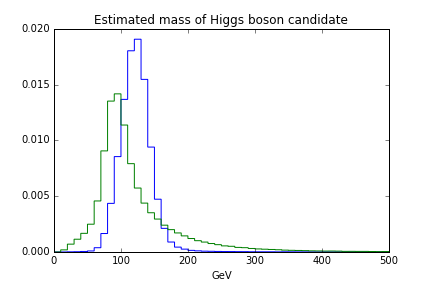
\includegraphics[width = 1.5in]{../plots/DER_mass_MMC.png}} &
\subfloat[]{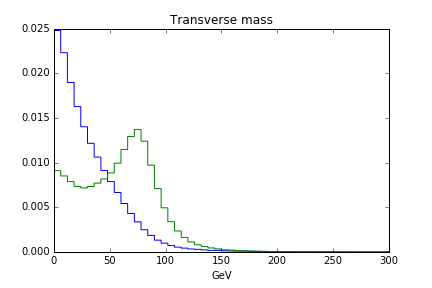
\includegraphics[width = 1.5in]{../plots/DER_mass_transverse_met_lep.png}} &
\subfloat[]{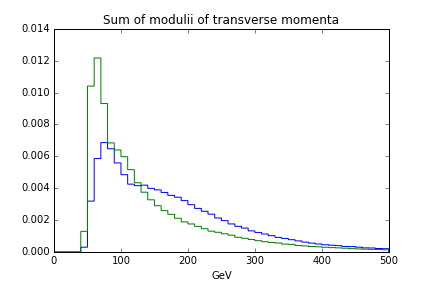
\includegraphics[width = 1.5in]{../plots/DER_sum_pt.png}}
\\
\subfloat[]{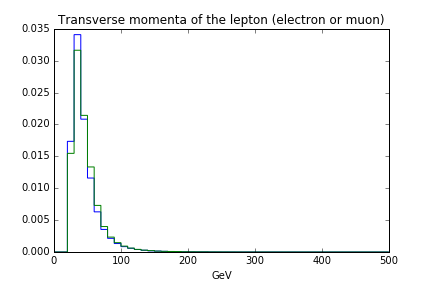
\includegraphics[width = 1.5in]{../plots/PRI_lep_pt.png}} &
\subfloat[]{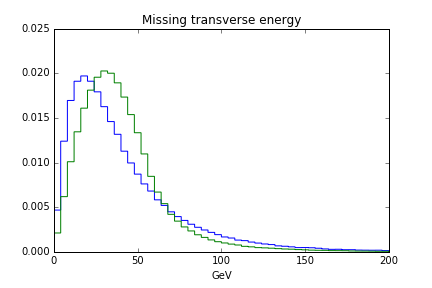
\includegraphics[width = 1.5in]{../plots/PRI_met.png}} &
\subfloat[]{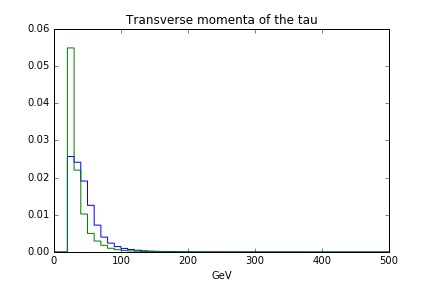
\includegraphics[width = 1.5in]{../plots/PRI_tau_pt.png}}
\\
\end{tabular}
\caption{Distributions of high level (top row) and low level(bottom row) features for signal (blue) and background (green) events. }
\label{fig:features_dist}
\end{center}
\end{figure}


Bayesian hyper-parameter optimization was conducted to minimized the cross entropy error of a neural network.  The hyper-parameters selected for optimization were the initial learning rate of the Adam optimizer, the number of hidden layers in the network, the number of hidden units per layer, and the weight decay constant.  Figure \ref{fig:hypers} gives the explored ranges of these hyper-parameters as well as the optimal values.  The ranges for the parameter were chosen to be similar to those used in \cite{Baldi:2014pta}. Optimization was implemented with the Spearmint software package.  A validation training set of 100,000 examples was used to train a model with the full feature set and then the cross entropy error was evaluated on a validation test set of 20,000 examples.  The optimization was allowed to proceed for 20 iterations of parameter selection and evaluation.  Ideally separate hyper-parameter optimizations would have been performed for the high-level, low-level and combinations of the low and high level features but due to computational limitations this was not possible. Hyper-parameters that were used without optimization were the mini-batch size of 100, the dropout probability of 0.50 and the choice of ReLU activations.  As shown in figure \ref{fig:hypers} a relatively small network was chosen with only two hidden layers and 150 units per hidden layer.  This is in stark contrast to \cite{Baldi:2014pta} where a similar Bayesian optimization was performed but the chosen network had 8 hidden layers with 500 hidden units per layer.  A separate hyper-parameter optimization was performed for a shallow network with the same parameter ranges but the number of hidden layers fixed at 1.  Once hyper-parameters were optimized they were used to train networks with three different feature sets using a training set size of 600,000 examples and then performance was evaluated on a test set of size 98,238.

\begin{figure}
\begin{center}
\tiny
 \begin{tabular}{|c| c c c|} 
 \hline
 Hyper-parameter & Minimum & Maximum & Optimal\\ [0.5ex] 
 \hline\hline
 Initial learning rate & 0.0001 & 1.0 & 0.0001 \\[1ex] 
 \hline
 Number of hidden units per layer & 50 & 500 & 150 \\[1ex]
 \hline
 Number of hidden layers & 2 & 8 & 2 \\[1ex]
 \hline
 Weight decay constant & 0.1 & 100 & 0.1 \\[1ex]
 \hline

\end{tabular}
\caption{Model hyper-parameters for DNN with their ranges and optimal values}
\label{fig:hypers}
\end{center}
\end{figure}

\begin{figure}
\begin{center}
\tiny
 \begin{tabular}{|c| c c c|} 
 \hline
 Hyper-parameter & Minimum & Maximum & Optimal\\ [0.5ex] 
 \hline\hline
 Initial learning rate & 0.0001 & 1.0 & 0.0001 \\[1ex] 
 \hline
 Number of hidden units per layer & 50 & 4000 & 800 \\[1ex]
 \hline
 Weight decay constant & 0.1 & 100 & 0.1 \\[1ex]
 \hline

\end{tabular}
\caption{Model hyper-parameters for shallow NN with their ranges and optimal values}
\label{fig:hypers}
\end{center}
\end{figure}

\subsection{results}

\begin{figure}
\begin{center}
\tiny
 \begin{tabular}{|c| c c|} 
 \hline
 Feature Set & Accuracy & AUC \\ [0.5ex] 
 \hline\hline
 High Level & 0.831 & 0.908 \\[1ex] 
 \hline
 Low Level & 0.807 & 0.876 \\[1ex]
 \hline
 All & 0.834 & 0.911 \\[1ex]
 \hline

\end{tabular}
\caption{Testing results by feature set for DNN}
\label{fig:results_dnn}
\end{center}
\end{figure}

\begin{figure}
\begin{center}
\begin{tabular}{cc}
\subfloat[]{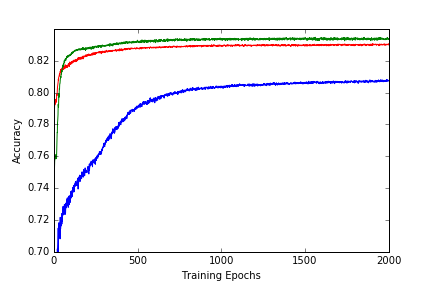
\includegraphics[width = 1.5in]{../plots/accuracy.png}} &
\subfloat[]{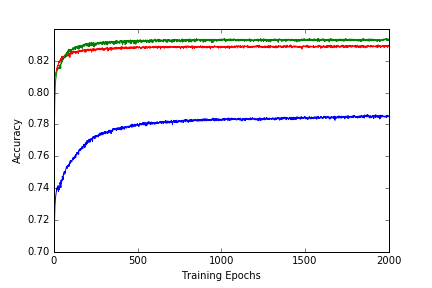
\includegraphics[width = 1.5in]{../plots/accuracy_nn.png}}
\end{tabular}
\caption{Accuracy by training epoch deep (a) and shallow (b) networks trained with high-level (red) low level (blue) and all (green) feature sets.}
\label{fig:accuracy}
\end{center}
\end{figure}

The test set results with for a deep network trained for 2000 epochs using the optimized hyper-parameters are summarized in figure \ref{fig:results_dnn} and the accuracy by training epoch is plotted in figure \ref{fig:accuracy}a.  It is apparent that best performance was achieved by a model trained on a combination of high level and low level features.  Furthermore  the worst performing model was trained on only the low level features.  This is in contrast to the results obtained in \cite{Baldi:2014pta} where deep networks trained on low level features achieved the same performance as those trained with high level features however in both cases the best performing models were trained on the full feature set.

Figure \ref{fig:results_nn} summarizes the results obtained during testing of the shallow network using an identical testing procedure to the one previously described.  Comparing figures \ref{fig:results_dnn} and \ref{fig:results_nn} it is apparent that there is almost no difference between the deep and shallow networks for models trained with the full feature set.  When only low level features are used the deep network outperformed the shallow network.  This is again in contrast to the results of \cite{Baldi:2014pta} where the deep network outperformed the shallow network in all cases.

\begin{figure}
\begin{center}
\tiny
 \begin{tabular}{|c| c c|} 
 \hline
 Feature Set & Accuracy & AUC \\ [0.5ex] 
 \hline\hline
 High Level & 0.829 & 0.909 \\[1ex] 
 \hline
 Low Level & 0.785 & 0.863 \\[1ex]
 \hline
 All & 0.834 & 0.912 \\[1ex]
 \hline

\end{tabular}
\caption{Testing results by feature set for shallow NN}
\label{fig:results_nn}
\end{center}
\end{figure}

\subsection{Conclusions and Future Work}
The previously described results indicate that training set size has several important implications on the performance of a neural network in a particle classification task.  The hyper-parameters selected by the Bayesian hyper-parameter optimization were very different in \cite{Baldi:2014pta} than those previously described.  This is likely because a much larger hyper-parameter validation set was used in the former case.  In \cite{Baldi:2014pta} hyper-parameters were optimized on a set of 40,000,000 examples whereas in this work it was only on  a set of 100,000.  With the more limited training set there was also no difference observed between the performance of the deep and shallow networks nor was the network trained with only low level features able to equal the performance of networks trained with high level features as was the case in \cite{Baldi:2014kfa}.

There are several potentially interesting extensions of this work that could be pursued.  While the dataset used in this work was composed of similar features to that of \cite{Baldi:2014pta} an alternative would have been to use a subset of that same dataset.  This would have made it easier to directly compare the performance of the model trained on the smaller dataset to models trained on the full dataset.  This work also did not explore the effect of certain hyper-parameter settings on model performance.  For example, the effects of different dropout probabilities could be investigated as well as other norm regularization techniques like $L_1$ or max norm.

{\small
\bibliographystyle{ieee}
\bibliography{egbib}
}

\appendix

\section{Dataset and implementation details}
Dataset available at \url{http://opendata.cern.ch/record/328?ln=en}.  Project code available at \url{https://github.com/jgartman/HiggsBosonML}.  Bayesian hyper-parameter optimization performed with Spearmint package \url{https://github.com/HIPS/Spearmint}.
\end{document}
